\documentclass[11pt]{article}

\usepackage[margin=1in]{geometry}
\usepackage{amsmath, amssymb, amsthm}
\usepackage{booktabs}
\usepackage{array}
\usepackage{tikz}
\usetikzlibrary{calc,arrows.meta,positioning}
\usepackage{xcolor}
\usepackage{hyperref}
\usepackage{enumitem}
\usepackage{microtype}
\usepackage{caption}
\usepackage{longtable}
\usepackage{mathtools}

\hypersetup{
    colorlinks=true,
    linkcolor=blue,
    citecolor=blue,
    urlcolor=blue
}

\setlength{\parskip}{0.65em}
\setlength{\parindent}{0pt}
\renewcommand{\arraystretch}{1.15}

\newtheorem{definition}{Definition}
\newtheorem{theorem}{Theorem}
\newtheorem{remark}{Remark}

\title{Envy-Free Rent Division:\\ Geometric Sperner Method and Maximin Optimization}
\author{Carlota Arzua}
\date{May 2026}

\begin{document}
\maketitle

\begin{abstract}
Rent division is a fair-division problem in which a group of people must assign rooms and split a fixed total rent. A desirable outcome should be \emph{envy-free}: no person should prefer another person's room at that room's assigned price. This report explains the mathematical model, develops a geometric algorithm based on Sperner's Lemma, and compares it with a maximin linear-programming algorithm. The geometric method is valuable because it gives an existence proof and a constructive approximation. The maximin optimization method is valuable because it is direct to implement when numerical valuations are available. A three-person worked example is used throughout.
\end{abstract}

\section{Introduction}

Fair division studies how to divide resources or costs among people who have different preferences. Rent division is a useful example because it combines an indivisible allocation problem with a divisible monetary transfer. The rooms are indivisible: each room must go to one person. The rent is divisible: room prices can be adjusted continuously as long as they add up to the total rent.

The central question is:

\begin{quote}
Given $n$ people, $n$ rooms, and a total rent $R$, can we assign each person one room and set room prices so that nobody wants to swap into another person's room at that other room's price?
\end{quote}

The answer is yes under standard assumptions. One route to this result uses Sperner's Lemma, a combinatorial-topological theorem about labelled triangulations of a simplex. Another route, once people give numerical valuations, is to solve a linear optimization problem.

This report separates the theory from the computation:

\begin{itemize}
    \item The \textbf{Sperner method} explains why envy-free rent divisions exist and how an approximate solution can be found by searching a triangulated price simplex.
    \item The \textbf{maximin linear-programming method} computes a solution from a valuation matrix and selects, among envy-free solutions, one that maximizes the utility of the worst-off person.
\end{itemize}

\section{Mathematical model}

Suppose there are $n$ people and $n$ rooms. Let
\[
    N=\{1,2,\dots,n\}
\]
be the set of people and rooms. The total rent is $R$.

A \emph{room assignment} is a permutation $\sigma$ of $N$. If $\sigma(i)=j$, then person $i$ receives room $j$.

A \emph{price vector} is
\[
    p=(p_1,p_2,\dots,p_n),
\]
where $p_j$ is the rent charged for room $j$. The prices must satisfy
\begin{equation}
    \sum_{j=1}^{n} p_j=R.
    \label{eq:pricesum}
\end{equation}

Depending on the model, one may also require $p_j\geq 0$ for all $j$. Some theoretical versions allow negative room prices. A negative price means that a person is being compensated to take a particularly undesirable room. This can be useful mathematically and sometimes economically, although many real rental agreements require nonnegative room prices.

\subsection{Quasi-linear utilities}

In the numerical model, each person reports how much each room is worth to them. Let
\[
    v_{ij}=\text{person } i\text{'s value for room }j.
\]
The utility person $i$ receives from room $j$ at price $p_j$ is
\begin{equation}
    u_{ij}=v_{ij}-p_j.
    \label{eq:utility}
\end{equation}

This is called a \emph{quasi-linear} model because money enters utility linearly. A room becomes more attractive when its personal value $v_{ij}$ is high and less attractive when its price $p_j$ is high.

A standard normalization is
\begin{equation}
    \sum_{j=1}^{n}v_{ij}=R \quad \text{for each person } i.
    \label{eq:normalization}
\end{equation}
This means each person distributes the total rent across the rooms according to how they value them. The algorithms still run without this normalization, but the interpretation is clearest when the totals equal the rent.

\begin{definition}[Envy-free rent division]
An assignment $\sigma$ and price vector $p$ are \emph{envy-free} if every person weakly prefers their assigned room to every other room at the listed prices:
\begin{equation}
    v_{i,\sigma(i)}-p_{\sigma(i)}\geq v_{ij}-p_j
    \quad \text{for every person }i\text{ and every room }j.
    \label{eq:envyfree}
\end{equation}
\end{definition}

The word \emph{weakly} matters. A tie is allowed. If a person is indifferent between their assigned room and another person's room, that is still envy-free.

\section{Worked example}

Consider three people and three rooms with total rent $R=1000$.

\begin{center}
\begin{tabular}{lrrr}
\toprule
\textbf{Room} & \textbf{Alice} & \textbf{Bob} & \textbf{Claire} \\
\midrule
Master Bedroom & 690 & 520 & 297 \\
Basement       &  95 & 333 & 633 \\
2nd Floor      & 215 & 147 &  70 \\
\midrule
Total          & 1000 & 1000 & 1000 \\
\bottomrule
\end{tabular}
\end{center}

One envy-free outcome is:

\begin{center}
\begin{tabular}{llr}
\toprule
\textbf{Person} & \textbf{Assigned room} & \textbf{Room price} \\
\midrule
Alice  & Master Bedroom & 488 \\
Bob    & 2nd Floor      &  13 \\
Claire & Basement       & 499 \\
\bottomrule
\end{tabular}
\end{center}

The prices add to the total rent:
\[
    488+13+499=1000.
\]

Now compute utilities using $u_{ij}=v_{ij}-p_j$.

\begin{center}
\begin{tabular}{lrrr}
\toprule
\textbf{Person} & \textbf{Master Bedroom} & \textbf{Basement} & \textbf{2nd Floor} \\
\midrule
Alice  & $690-488=202$  & $95-499=-404$   & $215-13=202$ \\
Bob    & $520-488=32$   & $333-499=-166$  & $147-13=134$ \\
Claire & $297-488=-191$ & $633-499=134$   & $70-13=57$ \\
\bottomrule
\end{tabular}
\end{center}

Alice is tied between the Master Bedroom and the 2nd Floor. Bob strictly prefers the 2nd Floor. Claire strictly prefers the Basement. Therefore, no person strictly prefers someone else's room at that other room's price, so the outcome is envy-free.

\section{The geometric Sperner method}

The geometric method represents price systems as points in a simplex. For three rooms, this simplex is a triangle. Each point in the triangle is one possible way to split the rent.

\subsection{The price simplex}

For three nonnegative prices, the price simplex is
\begin{equation}
    \Delta_R=\{(p_1,p_2,p_3):p_1+p_2+p_3=R,\;p_1,p_2,p_3\geq 0\}.
    \label{eq:pricesimplex}
\end{equation}

The three vertices are
\[
    (R,0,0),\quad (0,R,0),\quad (0,0,R).
\]
Each vertex puts the whole rent on one room. Each side makes one room free.

\begin{figure}[h]
\centering
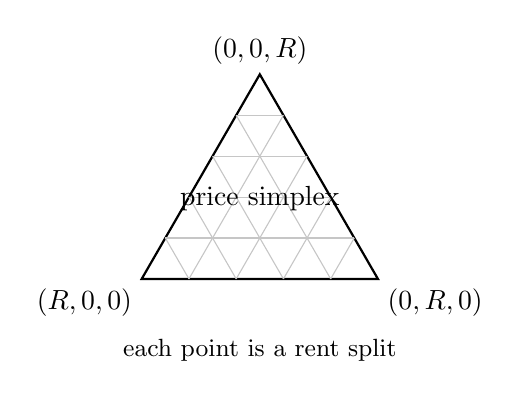
\begin{tikzpicture}[scale=3]
    \coordinate (A) at (0,0);
    \coordinate (B) at (1,0);
    \coordinate (C) at (0.5,0.866);

    \draw[thick] (A)--(B)--(C)--cycle;
    \node[below left] at (A) {$(R,0,0)$};
    \node[below right] at (B) {$(0,R,0)$};
    \node[above] at (C) {$(0,0,R)$};

    \foreach \t in {0.2,0.4,0.6,0.8} {
        \draw[gray!45] ($(A)!\t!(B)$) -- ($(C)!\t!(B)$);
        \draw[gray!45] ($(A)!\t!(C)$) -- ($(B)!\t!(C)$);
        \draw[gray!45] ($(B)!\t!(A)$) -- ($(C)!\t!(A)$);
    }

    \node at (0.5,0.34) {price simplex};
    \node[align=center, font=\small] at (0.5,-0.30) {each point is a rent split};
\end{tikzpicture}
\caption{For three rooms, all nonnegative price vectors that sum to $R$ form a triangle.}
\end{figure}

For $n$ rooms, the same object is an $(n-1)$-dimensional simplex:
\begin{equation}
    \Delta_R=\left\{p\in\mathbb{R}^n: \sum_{j=1}^{n}p_j=R,\;p_j\geq 0\right\}.
\end{equation}

\subsection{Preference labels}

At a price vector $p$, person $i$ chooses a room that maximizes utility:
\begin{equation}
    \operatorname{choice}_i(p)\in \arg\max_{j\in N}\{v_{ij}-p_j\}.
    \label{eq:choice}
\end{equation}

If there is a tie, any tied room can be chosen according to a fixed tie-breaking rule. In the geometric method, each vertex of the triangulation is assigned to one person. That person evaluates the prices at the vertex and labels the vertex by their preferred room.

For example, if a vertex is assigned to Alice and Alice's largest value of $v_{Aj}-p_j$ occurs at room 2, then that vertex receives label 2.

\subsection{Sperner's Lemma}

\begin{theorem}[Sperner's Lemma, two-dimensional version]
Triangulate a triangle into smaller triangles. Label each vertex with one of the three labels $1,2,3$. If the boundary labels satisfy Sperner's boundary condition--vertices on a side may only use the labels of that side's endpoints--then there exists at least one small triangle whose three vertices have labels $1,2,3$.
\end{theorem}

A small triangle with all three labels is called \emph{fully labelled} or \emph{panchromatic}. The importance of the theorem is that it guarantees existence. A fully labelled triangle must occur somewhere, regardless of how complicated the labelling is, as long as the boundary condition is satisfied.

\begin{figure}[h]
\centering
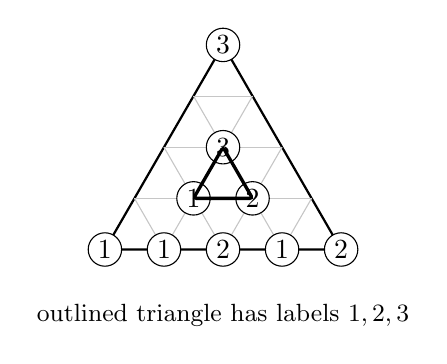
\begin{tikzpicture}[scale=3]
    \coordinate (A) at (0,0);
    \coordinate (B) at (1,0);
    \coordinate (C) at (0.5,0.866);
    \draw[thick] (A)--(B)--(C)--cycle;
    \foreach \t in {0.25,0.5,0.75} {
        \draw[gray!45] ($(A)!\t!(B)$) -- ($(C)!\t!(B)$);
        \draw[gray!45] ($(A)!\t!(C)$) -- ($(B)!\t!(C)$);
        \draw[gray!45] ($(B)!\t!(A)$) -- ($(C)!\t!(A)$);
    }
    \node[circle,draw,fill=white,inner sep=1.4pt] at (A) {1};
    \node[circle,draw,fill=white,inner sep=1.4pt] at (B) {2};
    \node[circle,draw,fill=white,inner sep=1.4pt] at (C) {3};
    \node[circle,draw,fill=white,inner sep=1.4pt] at (0.25,0) {1};
    \node[circle,draw,fill=white,inner sep=1.4pt] at (0.5,0) {2};
    \node[circle,draw,fill=white,inner sep=1.4pt] at (0.75,0) {1};
    \node[circle,draw,fill=white,inner sep=1.4pt] at (0.375,0.2165) {1};
    \node[circle,draw,fill=white,inner sep=1.4pt] at (0.625,0.2165) {2};
    \node[circle,draw,fill=white,inner sep=1.4pt] at (0.5,0.433) {3};

    \draw[line width=1.2pt, rounded corners=1pt] (0.375,0.2165)--(0.625,0.2165)--(0.5,0.433)--cycle;
    \node[font=\small,align=center] at (0.5,-0.28) {outlined triangle has labels $1,2,3$};
\end{tikzpicture}
\caption{Sperner's Lemma guarantees a small triangle with all three labels.}
\end{figure}

\subsection{How Sperner connects to rent division}

The rent division interpretation is:

\begin{center}
\begin{tabular}{>{\raggedright\arraybackslash}p{0.35\linewidth}>{\raggedright\arraybackslash}p{0.52\linewidth}}
\toprule
\textbf{Geometric object} & \textbf{Rent division meaning} \\
\midrule
Point in the simplex & A possible vector of room prices \\
Vertex of triangulation & A price vector that will be queried \\
Person assigned to a vertex & The person whose preference is checked there \\
Label of a vertex & The room that person prefers at those prices \\
Fully labelled small simplex & Nearby price vectors at which different people prefer different rooms \\
\bottomrule
\end{tabular}
\end{center}

The reason a fully labelled triangle matters is that its three labels represent the three rooms. If the vertices of this small triangle are also assigned to the three different people, then near that part of price space, Alice prefers one room, Bob prefers another, and Claire prefers the third. Because the vertices are close to one another, those preferences occur at nearly the same prices. This produces an approximate envy-free allocation.

As the triangulation becomes finer, the maximum distance between price vectors in one small triangle goes to zero. Therefore, the approximation improves. Under continuity assumptions on preferences, a limiting argument gives an exact envy-free price vector.

\subsection{Algorithm 1: triangulation search}

A computational version of the Sperner method can be written as follows.

\begin{center}
\fbox{%
\begin{minipage}{0.92\linewidth}
\textbf{Algorithm 1: Sperner-style rent division approximation}

\textbf{Input:} total rent $R$, people $1,\dots,n$, rooms $1,\dots,n$, valuation matrix $V=(v_{ij})$ or a preference oracle, mesh size $m$.

\begin{enumerate}[leftmargin=1.5em]
    \item Construct a grid on the price simplex. For $n=3$, use points
    \[
        \left(\frac{k_1R}{m},\frac{k_2R}{m},\frac{k_3R}{m}\right)
        \quad \text{where } k_1+k_2+k_3=m.
    \]
    \item Triangulate the grid into small simplices.
    \item Assign every vertex to one person, using a rule that makes each small simplex have one vertex for each person.
    \item At each vertex $p$, ask the assigned person to choose a favorite room. With numerical values, compute
    \[
        \arg\max_j\{v_{ij}-p_j\}.
    \]
    \item Label the vertex by that chosen room.
    \item Search the triangulation for a small simplex with all room labels $1,\dots,n$.
    \item Return the prices from that small simplex and assign people to the rooms indicated by the labels.
\end{enumerate}
\end{minipage}}
\end{center}

The output is approximate because the people may have made their choices at slightly different price vectors, namely the different vertices of the same small simplex. The approximation error is controlled by the mesh size $m$: larger $m$ means smaller triangles and more accurate prices.

\begin{remark}[Why a shifted price region can be useful]
In some rent-division examples, allowing negative room prices makes the model more flexible. Instead of the nonnegative simplex $p_j\geq 0$, one can search a shifted bounded region of price vectors satisfying $\sum_j p_j=R$. A large upper bound on prices forces at least one attractive low-price room on the boundary. This helps create the boundary behavior needed for a Sperner/Scarf-type argument. In an implementation, the same idea can be handled by choosing price bounds and checking the envy-free inequalities directly.
\end{remark}

\section{The maximin linear-programming method}

The geometric method is elegant, but a portfolio web app usually needs a fast and deterministic computational method. Once each person gives numerical values $v_{ij}$, envy-freeness becomes a system of linear inequalities.

\subsection{Fixed assignment problem}

Fix an assignment $\sigma$. The only unknowns are the room prices $p_1,\dots,p_n$. Envy-freeness requires
\[
    v_{i,\sigma(i)}-p_{\sigma(i)}\geq v_{ij}-p_j
\]
for every person $i$ and room $j$.

This inequality can be rearranged as
\begin{equation}
    p_{\sigma(i)}-p_j\leq v_{i,\sigma(i)}-v_{ij}.
    \label{eq:linearenvy}
\end{equation}
That is linear in the prices. Therefore, for a fixed assignment, checking whether the assignment can be made envy-free is a linear feasibility problem.

\subsection{Adding the maximin objective}

There may be many envy-free rent divisions. A fairness rule is needed to choose one. The \emph{maximin} rule chooses an envy-free outcome that maximizes the utility of the worst-off person.

Introduce a variable $t$ representing the minimum utility. For a fixed assignment $\sigma$, solve:

\begin{align}
    \text{maximize} \quad & t \\
    \text{subject to} \quad
    & \sum_{j=1}^{n}p_j=R, \label{lp:sum}\\
    & v_{i,\sigma(i)}-p_{\sigma(i)}\geq v_{ij}-p_j
    && \text{for all }i,j, \label{lp:envy}\\
    & v_{i,\sigma(i)}-p_{\sigma(i)}\geq t
    && \text{for all }i, \label{lp:minutil}\\
    & p_j\geq 0 \quad \text{if nonnegative prices are required.} \label{lp:nonnegative}
\end{align}

Constraint \eqref{lp:sum} makes prices add to the total rent. Constraint \eqref{lp:envy} enforces envy-freeness. Constraint \eqref{lp:minutil} makes $t$ a lower bound on each assigned utility. Maximizing $t$ improves the outcome for the person with the lowest utility.

\subsection{Algorithm 2: enumeration plus linear programming}

For small roommate problems, the easiest implementation is to check all possible assignments.

\begin{center}
\fbox{%
\begin{minipage}{0.92\linewidth}
\textbf{Algorithm 2: Maximin envy-free rent division}

\textbf{Input:} total rent $R$, people $1,\dots,n$, rooms $1,\dots,n$, valuation matrix $V=(v_{ij})$.

\begin{enumerate}[leftmargin=1.5em]
    \item Generate every room assignment $\sigma$.
    \item For each assignment, solve the linear program \eqref{lp:sum}--\eqref{lp:nonnegative}.
    \item Discard assignments for which the linear program is infeasible.
    \item Among feasible assignments, choose the one with the largest optimal value of $t$.
    \item Return the assignment, the prices, and a utility table verifying envy-freeness.
\end{enumerate}
\end{minipage}}
\end{center}

The enumeration cost is $n!$ assignments. This is fine for typical roommate settings:
\[
3!=6,\quad 4!=24,\quad 5!=120,\quad 6!=720.
\]
For much larger instances, one would use more advanced optimization techniques rather than naive enumeration.

\subsection{Applying the LP idea to the example}

For the assignment
\[
    \sigma(\text{Alice})=\text{Master Bedroom},\quad
    \sigma(\text{Bob})=\text{2nd Floor},\quad
    \sigma(\text{Claire})=\text{Basement},
\]
the envy-free constraints include the following inequalities.

For Alice:
\begin{align*}
690-p_M &\geq 95-p_B,\\
690-p_M &\geq 215-p_2.
\end{align*}

For Bob:
\begin{align*}
147-p_2 &\geq 520-p_M,\\
147-p_2 &\geq 333-p_B.
\end{align*}

For Claire:
\begin{align*}
633-p_B &\geq 297-p_M,\\
633-p_B &\geq 70-p_2.
\end{align*}

Together with
\[
    p_M+p_B+p_2=1000,
\]
these constraints describe the price region that makes this assignment envy-free. The solution
\[
    p_M=488,
    \quad p_B=499,
    \quad p_2=13
\]
satisfies the inequalities and gives minimum assigned utility
\[
    \min\{202,134,134\}=134.
\]

\section{Comparison of the two algorithms}

\begin{longtable}{>{\raggedright\arraybackslash}p{0.24\linewidth}>{\raggedright\arraybackslash}p{0.34\linewidth}>{\raggedright\arraybackslash}p{0.34\linewidth}}
\toprule
\textbf{Feature} & \textbf{Sperner / geometric method} & \textbf{Maximin / linear-programming method} \\
\midrule
Main object
& A triangulated simplex of price vectors.
& A system of linear inequalities in room prices. \\
\addlinespace
Type of input
& Can be based on preference queries: ``Which room do you choose at these prices?''
& Requires numerical valuations $v_{ij}$ for every person and room. \\
\addlinespace
Main guarantee
& A fully labelled small simplex exists, leading to an approximate envy-free outcome.
& A computed solution is envy-free for the reported valuation matrix, up to numerical solver precision. \\
\addlinespace
Fairness selection
& Primarily an existence and approximation method; it may find one of many envy-free outcomes.
& Selects a particular envy-free outcome by maximizing the minimum assigned utility. \\
\addlinespace
Accuracy
& Depends on the triangulation mesh size. Finer mesh gives better approximation.
& Exact for the linear model, subject to numerical precision. \\
\addlinespace
Interpretability
& Strong visual interpretation: prices live in a triangle and labels show preferred rooms.
& Strong computational interpretation: each fairness requirement is an inequality. \\
\addlinespace
Best use
& Explaining why a fair rent split exists and visualizing the topology behind fair division.
& Building a practical calculator or web app from numerical inputs. \\
\addlinespace
Limitation
& May require many preference queries for high accuracy.
& Assumes quasi-linear utilities and truthful numerical valuations. \\
\bottomrule
\end{longtable}

The two methods are not contradictory. They are two different ways of searching the same kind of object: prices that support an envy-free assignment. The Sperner method searches geometrically by labelling a triangulation. The LP method searches algebraically by imposing the envy-free inequalities directly.

\section{What the implementation computes}

The Python implementation in this project follows Algorithm 2. It does not simulate the full Sperner triangulation search. Instead, it uses the numerical model directly:
\[
    u_{ij}=v_{ij}-p_j.
\]

The program:

\begin{enumerate}
    \item reads a valuation matrix,
    \item enumerates room assignments,
    \item solves a linear program for each assignment,
    \item chooses the feasible assignment with the largest minimum utility,
    \item displays the final assignment, prices, and envy-check table.
\end{enumerate}

This makes the implementation appropriate for a portfolio project because it has clear input, output, and verification. The Sperner method remains important because it explains the deeper mathematical reason that envy-free rent divisions exist.

\section{Possible extensions}

Several extensions could make the project stronger.

\begin{itemize}
    \item \textbf{Sperner visualization:} add an interactive triangle showing price points, preference labels, and a fully labelled small triangle.
    \item \textbf{MATLAB implementation:} implement the same LP using MATLAB's \texttt{linprog} to show the optimization model in another language.
    \item \textbf{Different fairness rules:} compare maximin with other envy-free solutions, such as minimizing price spread or maximizing total assigned utility.
    \item \textbf{Tie handling:} explicitly show ties in the output and explain why ties do not violate envy-freeness.
    \item \textbf{Price bounds:} let the user choose whether room prices must be nonnegative or whether negative prices are allowed.
\end{itemize}

\section{Conclusion}

Rent division is mathematically rich because it combines discrete assignment, continuous prices, and fairness constraints. The Sperner method gives a geometric explanation: triangulate the price simplex, label vertices by preferred rooms, and use a fully labelled simplex to locate an approximately envy-free rent split. The maximin linear-programming method gives a practical computation: encode envy-freeness as inequalities and choose the solution that maximizes the minimum utility.

For a portfolio, the strongest presentation is to describe both layers. The geometric method shows theoretical depth. The LP implementation shows that the theory can be turned into working code.

\begin{thebibliography}{9}

\bibitem{su1999}
Francis Edward Su.
\newblock \emph{Rental Harmony: Sperner's Lemma in Fair Division}.
\newblock American Mathematical Monthly, 106(10):930--942, 1999.
\newblock \url{https://www.cs.cmu.edu/~arielpro/15896s16/docs/paper11a.pdf}

\bibitem{gal2017}
Ya'akov (Kobi) Gal, Moshe Mash, Ariel D. Procaccia, and Yair Zick.
\newblock \emph{Which Is the Fairest (Rent Division) of Them All?}
\newblock Journal of the ACM, 64(6), Article 39, 2017.
\newblock \url{https://doi.org/10.1145/3131361}

\bibitem{spliddit}
Spliddit.
\newblock \emph{Fair Division of Rent, Goods, Credit, Fare, and Tasks}.
\newblock \url{https://www.spliddit.org/}

\end{thebibliography}

\end{document}
